\subchapter{Configuring pin muxing}
{Objective: learn how to declare and use a muxing state.}

\section{Goals}

As part of the previous lab, we enabled an I2C controller and described
a device plugged on the bus. In this lab we will cover how to ensure a
proper communication between the two and be able to declare and use
pinctrl settings.

\section{Setup}

Continue using the \code{bootlin-labs} branch in the
\code{~/linux-kernel-labs/src/linux} directory.

\section{Probing the different busses}

Now, let's use \code{i2cdetect}'s capability to probe a bus for
devices. The I2C bus has no real discovery capability, but yet, the tool
exploits a feature of the specification: when the master talks to a
device, it starts by sending the target address on the bus and expects
it to be acked by the relevant device. Iterating through all the
possible addresses without sending anything after the address byte,
looking for the presence of an Ack is what uses the tool to probe the
devices. That is also why we get a warning when using it.

Let's start by probing the bus associated to \code{i2c-0}:

\begin{bashinput}
# i2cdetect -r 1
i2cdetect: WARNING! This program can confuse your I2C bus
Continue? [y/N] y
     0  1  2  3  4  5  6  7  8  9  a  b  c  d  e  f
00:          -- -- -- -- -- -- -- -- -- -- -- -- -- 
10: -- -- -- -- -- -- -- -- -- -- -- -- -- -- -- -- 
20: -- -- UU -- -- UU -- -- -- -- -- -- -- -- -- -- 
30: -- -- -- -- -- -- -- -- -- -- -- -- -- -- -- -- 
40: -- -- -- -- -- -- -- -- -- -- -- -- -- -- -- -- 
50: 50 -- -- -- -- -- -- -- -- -- -- -- -- -- -- -- 
60: -- -- -- -- -- -- -- -- -- -- -- -- -- -- -- -- 
70: -- -- -- -- -- -- -- --     
\end{bashinput}

We can see three devices on this internal bus:
\begin{itemize}
\item Two at address \code{0x22} and \code{0x25}, indicated by \code{UU},
      which means that there is a kernel driver actively
      driving these devices.
\item One other device at addresses \code{0x50}.
      We just know that is currently not bound to a kernel driver.
\end{itemize}

Now try to probe I2C4 with \code{i2cdetect -r 3}.

You will see that the command will fail to connect to
the bus. That's because the corresponding signals are
not propely muxed, yet.

\section{Find pin muxing configuration information for i2c4}

As you found in the previous lab, we now managed to have our nunchuk
device enumerated on the \code{lpi2c4} bus.

However, to access the bus data and clock signals, we need to configure
the pin muxing of the SoC.

To this end, NXP provides ready-made configurations for the i.MX93 SoC.
You can refer to the imx93-pinfunc.h file, which contains a list of predefined macros used to configure the pin multiplexing.

By searching for \code{LPI2C4}, we find the macros \code{MX93_PAD_GPIO_IO02__LPI2C4_SDA} and \code{MX93_PAD_GPIO_IO03__LPI2C4_SCL}, which allow us to multiplex the \code{GPIO_IO02} and \code{GPIO_IO03} pins as \code{LPI2C4_SDA} and \code{LPI2C4_SCL}, respectively.

For more information on the multiplexing values, you can refer to the i.MX93 processor reference manual, in the
{\em IOMUX Controller (IOMUXC)} section.

Now that we have our multiplexing macros, we still need to define the pad control value.
We will use the same value that is used for the other I2C buses, namely \code{0x40000B9E}.Here, this means that the pad control is configured with a fast slew rate, in pull-up mode, with a drive strength equivalent to X4, in open-drain mode, and without a Schmitt trigger input.
For more details on pad control values, you can also refer to the
{\em IOMUX Controller (IOMUXC)} section in the i.MX93 processor reference manual.

\section{Multiplexing the I2C controller outputs correctly}

Now that we have all the necessary information, we can use the definition of \code{LPI2C1} as a reference to build our own \code{pinctrl} node.
It is also helpful to look into other \code{.dts} files to see how the other I2C buses are defined. So in our case it should look like this:

{\small
\begin{verbatim}
pinctrl_lpi2c4: lpi2c4grp {
      fsl,pins = <
            MX93_PAD_GPIO_IO03__LPI2C4_SCL                  0x40000b9e
            MX93_PAD_GPIO_IO02__LPI2C4_SDA                  0x40000b9e
      >;
};
\end{verbatim}
}

Now that pin muxing settings have been explained, edit your board
DTS file to add the same definitions to enable pin muxing for \code{lpi2c4}.
Don't forget that you don't have to repeat definitions that are
already present in the \code{.dtsi} files. Just add new declarations, or
settings that override existing definitions.

Rebuild and update your DTB, and eventually reboot the board. You should
now be able to probe your bus:

\begin{bashinput}
# i2cdetect -r 3
i2cdetect: WARNING! This program can confuse your I2C bus
Continue? [y/N] y
     0  1  2  3  4  5  6  7  8  9  a  b  c  d  e  f
00:          -- -- -- -- -- -- -- -- -- -- -- -- --
10: -- -- -- -- -- -- -- -- -- -- -- -- -- -- -- --
20: -- -- -- -- -- -- -- -- -- -- -- -- -- -- -- --
30: -- -- -- -- -- -- -- -- -- -- -- -- -- -- -- --
40: -- -- -- -- -- -- -- -- -- -- -- -- -- -- -- --
50: -- -- -- -- -- -- -- -- -- -- -- -- -- -- -- --
60: -- -- -- -- -- -- -- -- -- -- -- -- -- -- -- --
70: -- -- -- -- -- -- -- --
\end{bashinput}

No devices are detected, because we did not wire the nunchuk yet.

\subsection{Wiring the I2C device}

Let's connect the Nunchuk provided by your instructor
to the I2C4 bus on the board, using breadboard wires:

\includegraphics[width=0.3\textwidth]{common/nunchuk-pinout.pdf}
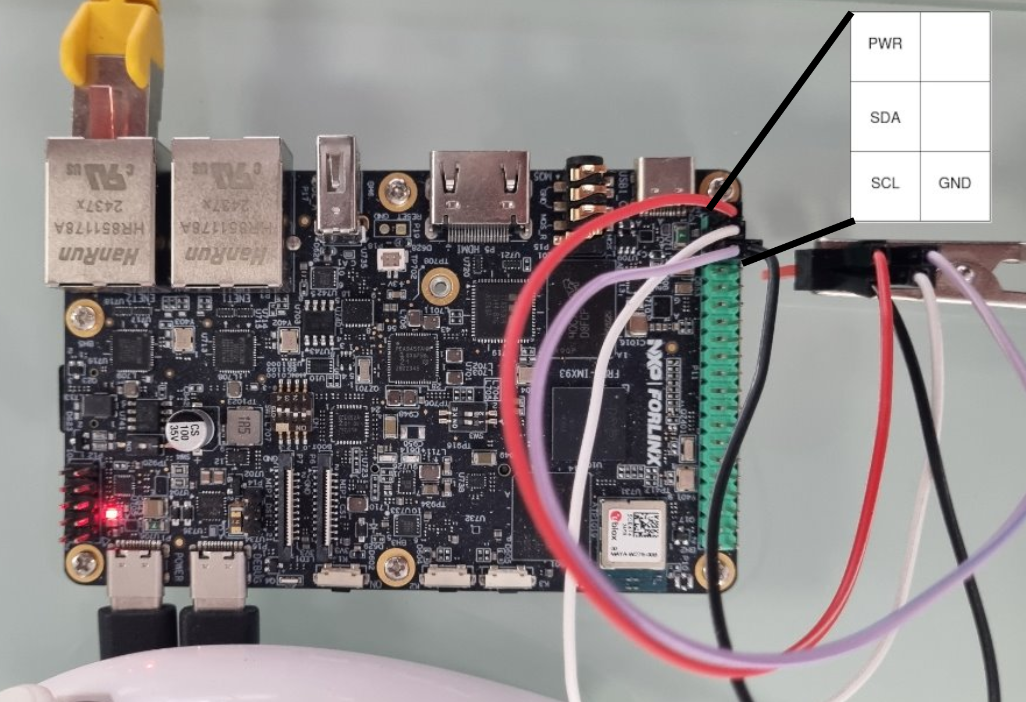
\includegraphics[width=0.7\textwidth]{labs/kernel-i2c-multiplexing-imx93-frdm/imx93-frdm-connect-nunchuk.png}

\begin{itemize}
\item Connect the Nunchuk PWR pin to pin 1 (3V3) of connector P11
\item Connect the Nunchuk GND pin to pin 6 (GND) of connector P11
\item Connect the Nunchuk SCL pin to pin 5 of connector P11
\item Connect the Nunchuk SDA pin to pin 3 of connector P11
\end{itemize}

If you didn't do any mistake, your new device should be detected at
address \code{0x52}:

\begin{bashinput}
# i2cdetect -r 3
i2cdetect: WARNING! This program can confuse your I2C bus
Continue? [y/N] y
     0  1  2  3  4  5  6  7  8  9  a  b  c  d  e  f
00:          -- -- -- -- -- -- -- -- -- -- -- -- --
10: -- -- -- -- -- -- -- -- -- -- -- -- -- -- -- --
20: -- -- -- -- -- -- -- -- -- -- -- -- -- -- -- --
30: -- -- -- -- -- -- -- -- -- -- -- -- -- -- -- --
40: -- -- -- -- -- -- -- -- -- -- -- -- -- -- -- --
50: -- -- 52 -- -- -- -- -- -- -- -- -- -- -- -- --
60: -- -- -- -- -- -- -- -- -- -- -- -- -- -- -- --
70: -- -- -- -- -- -- -- --
\end{bashinput}

We will later compile an out-of-tree kernel module to support this device.
